\documentclass[../main.tex]{subfiles}
\graphicspath{{resources/}{resources/pcb_res}}
 
\begin{document}

\section{Tervezési feladat követelményeinek felállítása}
    A feladatot az Ebay-en vásárolt olcsó modulok segítségével szerettem volna megvalósítani, amik már a rendelkezésemre álltak. A cél egy olyan áramköri elem megépítése volt, ami viszonylag könnyedén beforrasztható, külső egyenáramú tápellátásról vezérelni tudja a rákapcsolt LED sorokat, és egy cserélhető Wifi modulon keresztül képes az Androidos alkalmazásunkból érkező, általam definiált protokollú, adatok fogadására. Továbbá egy olyan védődoboz tervezése, amivel különböző helyekre lehet majd felszerelni. A következőkben pontokba szedtem az összes tervezési követelményt:
 
        \begin{itemize}
            \item Legyen telefonnal működtethető vezeték nélküli hálózaton keresztül
            \item Rendelkezésre álló modulokból épüljön fel
            \item Legyen minél kisebb, de még kézzel beforrasztható
            \item Védve legyen a külső behatások ellen (védődoboz)
            \item Legyen hordozhatóvá tehető, akkumulátorról működtethető
            \item Tápfeszültségek szempontjából
                 \begin{itemize}
                    \item 12V DC tápfeszültség a LED sor számára
                    \item 3,3V DC tápfeszültség a mikrovezérlő és a Wifi-modul számára
                    \item 5V DC tápfeszültség a mikrovezérlőből kijövő 3,3V jelének 5V-sra alakításához
                \end{itemize}
        \end{itemize}
    
    
    \subsection{Rendelkezésre álló hardverek}
        \subsubsection{Wifi modul: ESP8266 - ESP01} 
            Az ESP8266 egy olyan IC, ami IoT világnak\cite{a_iot} megfelelően lett tervezve. Képes egy 802.11 típusú hálózaton TCP/IP protokoll segítségével kommunikálni. Teljesen címezhető SPI vagy UART segítségével, és hozzáférést ad a GPIO-hoz.\cite{sec_201} \\[12px]
            Néhány tulajdonsága:
            \begin{itemize}
                \item 802.11 b/g/n szabványokat támogat
                \item Wi-Fi Direct (P2P), soft-AP módú működés
                \item integrált TCP/IP protokoll
                \item integrált WEP, TKIP, AES motorok
                \item 3.3V DC tápfelszültség
            \end{itemize}
            
            Ennek az IC-nek az ESP01 típusú modulját (\ref{fig:esp01}. Ábra) használtam. Körülbelül 500 Ft-ért lehet hozzájutni az Ebay-en, és egy 2x4-es csatlakozóval lehet az áramkörünkhöz csatlakoztatni.
            
            \begin{figure}[h!]
                \centering
                    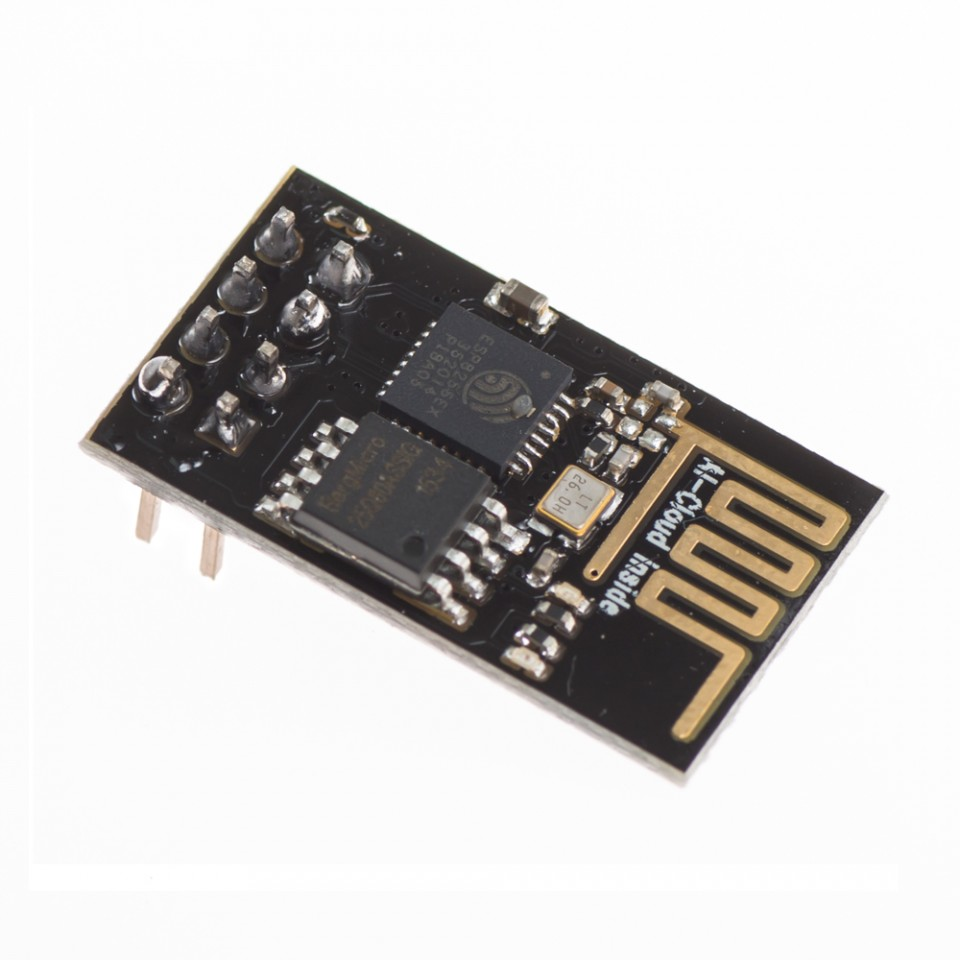
\includegraphics[width=5cm]{resources/pcb_res/esp01.jpg}
                \caption{ESP01-es Wifi Modul\cite{sec_201}}
                \label{fig:esp01}
            \end{figure}
        
        \subsubsection{WS2811-es IC-vel ellátott címezhető LED szalag}
            
            \begin{figure}[h!]
                \centering
                    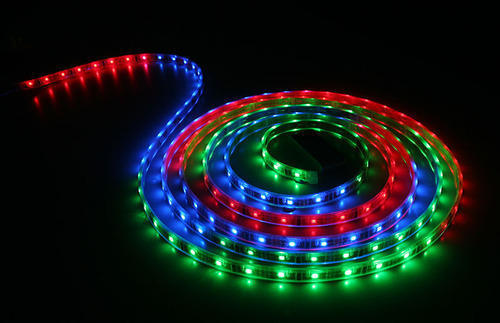
\includegraphics[width=7cm]{resources/pcb_res/ledstrip}
                \caption{Ebay-ről vásárolt LED szalag}
                \label{fig:ledstrip}
            \end{figure}
        
            A WS2811 egy 3 kimeneti csatornás speciális LED meghajtó IC. Egy jelvezetéken küldött 24 bit szélességű bitsorozattal lehet vezérelni 400 vagy 800 Kbps sebességgel. Az IC-ben van belső jelerősítő, hogy egymás után lehessen kötni őket. Az általam vásárolt LED szalagon IC-nként 3 db] RGB LED található, és ezek az IC-k az imént említett módon vannak összekötve. Ezt a felépítést szemlélteti \aref{fig:ledstrip_schematic}.~ábra.\\[12px]
            
            \begin{figure}[h!]
                \centering
                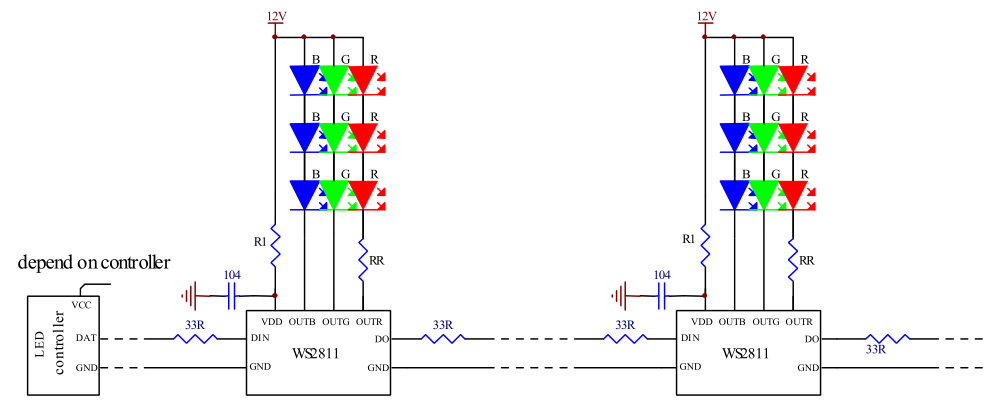
\includegraphics[width=14cm]{resources/pcb_res/ledstrip_schematic.png}
                \caption{Ebay-ről vásárolt LED szalag felépítése\cite{ds_ws2811}}
                \label{fig:ledstrip_schematic}
            \end{figure}
            
            LED szalag tulajdonságai:
            \begin{itemize}
                \item 12V DC tápfeszültség
                \item 1 A maximális áramfelvétel
                \item 5V-os jelvezeték
                \item 5 $m$ hosszú, 150 RGB LED-et tartalmaz
                \item 3 RGB LED/IC
            \end{itemize}
            
        \subsubsection{Mikrovezérlő: STM32F103C8T6}
            Ez a mikrovezérlő az F103-as család tagja, azon belül pedig az a változat, aminek 48 lába van (C), 64 Kbyte Flash memóriája van (8), LQFP csomagú (T) és -40-től +85°C-ig működik (6). \cite{ds_stm32}
            
            \begin{figure}[h!]
                \centering
                    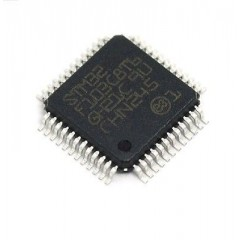
\includegraphics[width=4.5cm]{resources/pcb_res/stm32f103c8t6.jpg}
                \caption{STM32F103C8T6 típusú mikrovezérlő\cite{sec_204}}
                \label{fig:stm32f103_ic}
            \end{figure}
            
            Egy maximum 72 MHz-es, 32-bit-es ARM Cortex-M3-as processzor a magja, ami a fent említett Flash és SRAM memória és megannyi más egység (2x A/D konverter, DMA vezérlő 37 I/O port, 7x timer, és 9 kommunikációs interfész) is kiegészít. Számomra az időzítők (PWM generálás, és időzítési feladatok), az UART interfész és a DMA vezérlő játszik fontos szerepet, illetve az A/D konverterek bővítési lehetőségként.
            
            \begin{figure}[h!]
                \centering
                    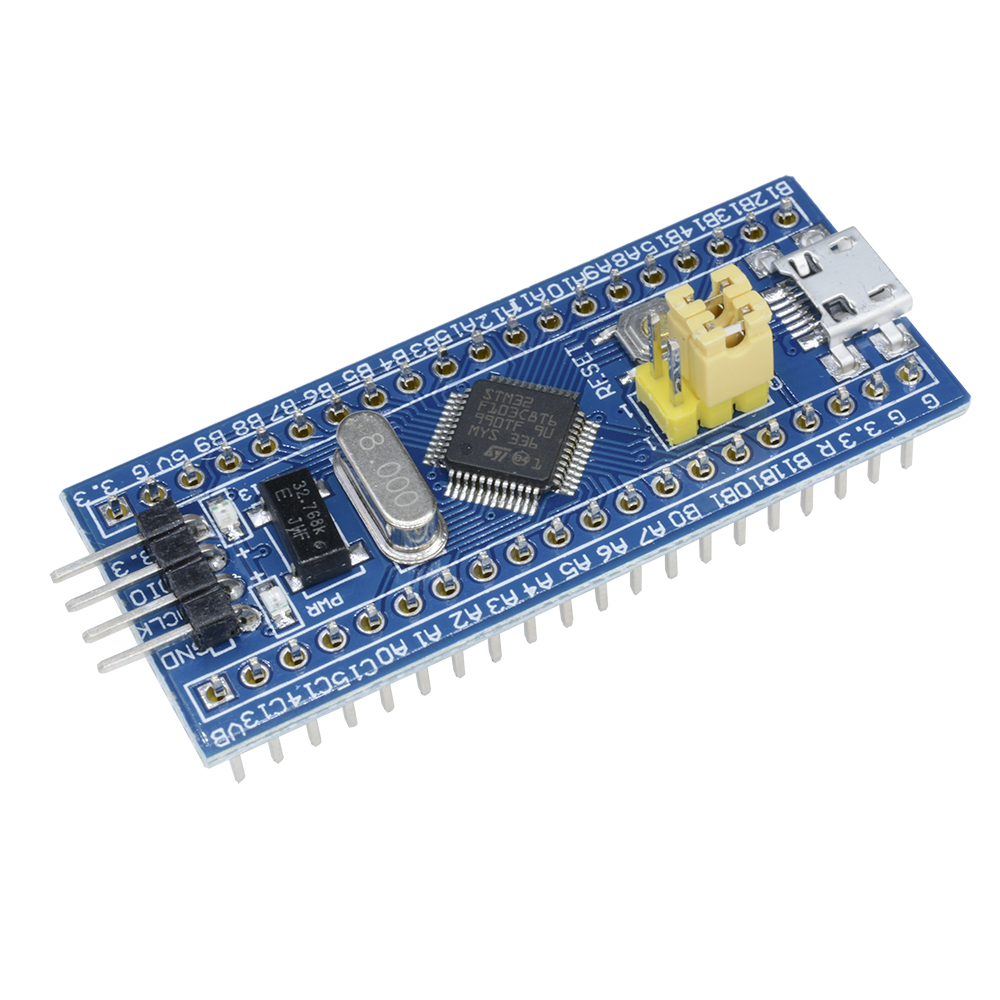
\includegraphics[width=7cm]{resources/pcb_res/stm32f103c8t6_minimum_dev_board.jpg}
                \caption{Ebay-ről vásárolt STM32F103C8T6-es minimum fejlesztői lap\cite{sec_205}}
                \label{fig:stm32f103_dev_board}
            \end{figure}

\newpage

\end{document}
